% !TeX spellcheck = en_GB
%\begin{wrapfigure}{r}{0.6\textwidth}
\begin{figure}[t!]
	\centering
	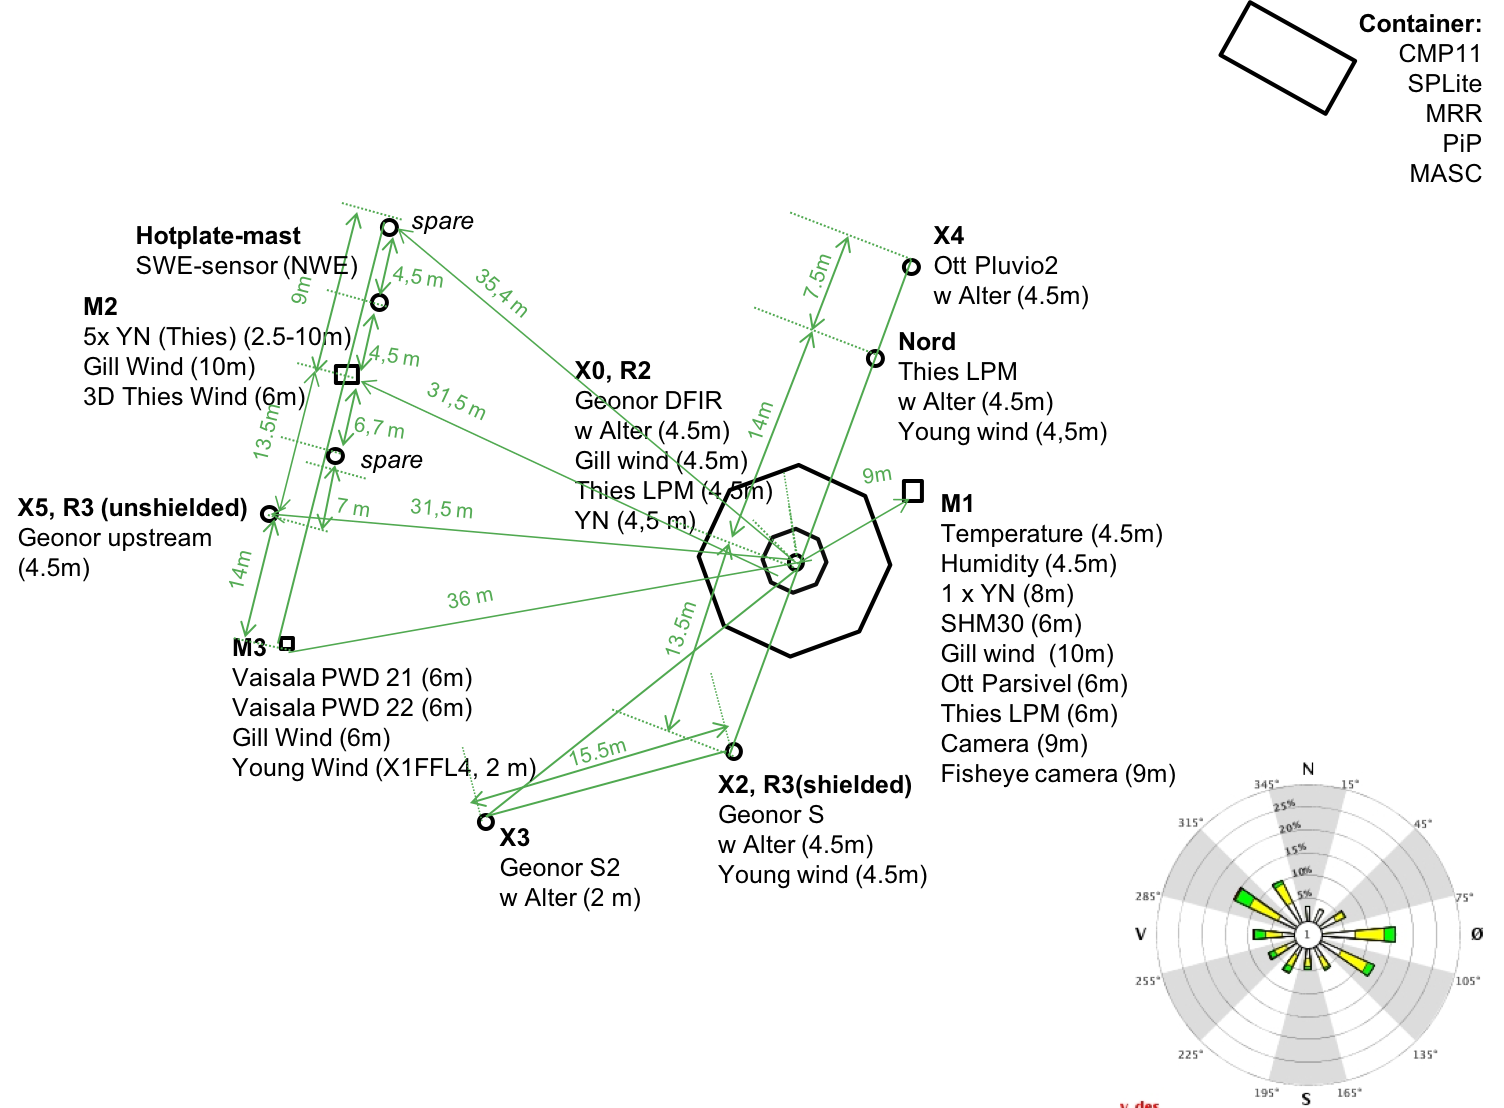
\includegraphics[width=0.9\textwidth]{./fig_instruments/instrument_setting.png}
	%	\vspace{-10pt}
	\caption{Instrument setting at the Haukeliseter measurement site during winter 2016/2017. \textbf{X0}, Double fence gauge (double octagon), \textbf{M1}, weather mast with pressure, temperature and \SI{10}{\metre} wind sensor. \textbf{Container}, with Micro Rain Radar, Particle Imaging Package, and Multi-Angular Snowfall Camera. The windrose indicates the mean wind direction from either from west-north-west or east-south-east averaged from three winters \citep[adapdet from][]{wolff_derivation_2015}. }\label{fig:inst_setting}
\end{figure}
%	\vspace{-\normalbaselineskip}

%	\vspace{-\normalbaselineskip}
%\end{wrapfigure}